\section{Envelope Shapers}

El <<generador de envolvente>> (conocido por sus nombres en inglés, \textit{Envelope Shaper} o \textit{Envelope Generator}), es uno de los módulos, junto con el de los osciladores, que no suelen faltar en los sintetizadores analógicos. Pero esta omnipresencia no es paralela a su estandarización. Los parámetros que controlan el generador de envolvente dependen de cada fabricante e, incluso, de cada modelo. Por si fuera poco, precisamente una de las grandes diferencias entre el Synthi 100 de Cuenca y el resto de Synthi 100 son los parámetros del módulo \textit{Envelope Shaper}que este permite variar, lo cual da fe de la velocidad a la que el concepto de envolvente se desarrollaba por aquellos años.

\subsection{Las fases de una envolvente típica}

Una <<envolvente>> puede ser descrita como la forma que se da al desarrollo en el tiempo del nivel de un parámetro de una señal, habitualmente la amplitud. De esta forma, una señal continua generada, por ejemplo, con un oscilador, puede adquirir una evolución dinámica, así como un inicio y un final. Puesto que una envolvente puede <<envolver>> a cualquier tipo de señal, sea esta de audio como de voltaje, podemos hacer variar con ella otros parámetros como la frecuencia de un oscilador, la frecuencia de corte de un filtro, el nivel de salida de otra envolvente, etc.

Históricamente, la envolvente surge inspirada por el comportamiento físico de los instrumentos musicales (IMAGEN: FORMA DE ONDA NOTA PIANO), de ahí que el tipo de envolvente más popular hasta nuestros días es el ADSR, siglas de los términos en inglés \textit{attack}, \textit{decay}, \textit{sustain} y \textit{release} (Fig. \ref{fig:adsr}):
\begin{description}
	\item[\textit{Attack}] Tiempo transcurrido entre el nivel 0 y el punto álgido (convencionalmente 1). Es el equivalente al \textit{ataque} de un instrumento acústico tipo, en el que los sonidos transitorios pueden producir un rápido pico dinámico.
	\item[\textit{Decay}] Tiempo transcurrido entre el final del ataque, con nivel 1 y el nivel de \textit{sustain}. En instrumentos acústicos, tras alcanzar el nivel máximo en el periodo de ataque, existe un progresivo \textit{decaimiento} dinámico del sonido hasta alcanzar un nivel estable.
	\item[\textit{Sustain}] Nivel en el que la señal puede ser mantenida por tiempo indefinido (entre 0 y 1). A diferencia del resto de parámetros, el \textit{sustain} no es un parámetro temporal, sino de nivel. De hecho, es el único parámetro de nivel de toda la envolvente, ya que el nivel inicial y final siempre son 0 mientras que el nivel alcanzado en el ataque siempre es 1 (entendiendo estos valores como factor de cualquier unidad de medida). En los instrumentos acústicos, este nivel es mantenido a voluntad por el instrumentista. En los sintetizadores (analógicos o digitales) se utiliza el control de \textit{gate} para mantener la señal en \textit{sustain}.
	\item[\textit{Release}] Tiempo transcurrido entre el final del mantenimiento de la señal (\textit{sustain}), y su extinción. 
\end{description} 

\begin{figure}
	\centering
	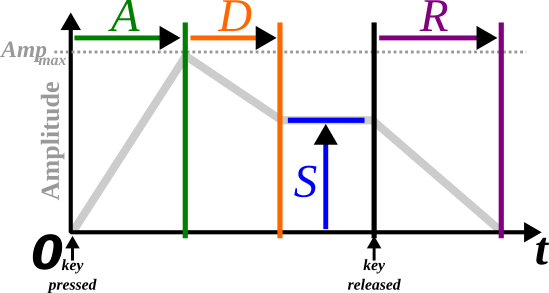
\includegraphics[width=0.7\textwidth]{env_ADSR}
	\caption{Esquema de una envolvente tipo ADSR.}
	\label{fig:adsr}
\end{figure}

\subsection{Control de la envolvente: \textit{Gate} y \textit{trigger}}

Como se ha indicado, \textit{attack}, \textit{decay} y \textit{release} son duraciones, con lo que su inicio y fin están determinados por los valores elegidos por el usuario (o por el control desde otro módulo), pero ¿cómo sabe el sintetizador cuándo ha de terminar \textit{sustain} y comenzar el periodo de \textit{release}? Y otra pregunta muy relacionada, ¿cómo se da comienzo al periodo de \textit{attack}? La analogía de un instrumento de tecla, como el órgano, puede darnos una respuesta muy intuitiva: Cuando el organista baja la tecla se pone en marcha el ciclo completo de la nota musical con su propia envolvente dinámica. En ese preciso instante comienza un periodo de crecimento sonoro producido por el propio aire entrando a los tubos como por las sucesivas reflexiones del sonido recién comenzado en las paredes de la sala. Tanto el \textit{ataque} como el \textit{decaimiento} tienen lugar con un tiempo definido para cada tubo, con controlable por el intérprete. Una vez estabilizado el sonido en un nivel determinado (\textit{sustain}) el sonido continuará este nivel tanto tiempo como quiera el intérprete. Solo cuando levante la tecla a su posición inicial será cuando se de comienzo a la fase de \textit{release}, en la que el sonido, dependiendo de las características de la sala, requerirá de un periodo de tiempo mayor o menor hasta dejar de ser escuchado.

La tecla \textit{bajada} y \textit{subida} tiene su análogo dentro del mundo de los sintetizadores en el concepto de \textit{gate} (\textit{<<puerta>>}), la cual se puede encontrar, del mismo modo, en dos estados: \textit{abierta} (valor mayor que 0) y \textit{cerrada} (valor de 0 o inferior). El valor de este \textit{gate} no es otra cosa que un nivel de voltaje en el caso de los sintetizadores analógicos o el valor digital de 1 o 0 en el caso de un dispositivo de \textit{software}. En ambos casos, \textit{gate} puede ser considerada otra señal, cuya función es la de <<dirigir>> las etapas de la envolvente. 

Si la señal \textit{gate} viene delimitada por su inicio y su fin ---puntos con los que se ponen en marcha los diferentes periodos de una envolvente--- el \textit{trigger} es cualquier señal cuando pasa de un valor de 0 o negativo hasta un valor positivo. Es el inicio de dicha señal (momento en el que pasa a ser mayor que 0) el que puede ser usado como \textit{trigger}. Para el desarrollo de una envolvente en la que no existe \textit{sustain} bastaría una señal \textit{trigger} para dar el <<pistoletazo de salida>> y recorrer sucesivamente todas sus etapas de principio a fin, con una duración total suma de todas ellas: \textit{attack}, \textit{decay} y \textit{release}. 


FIGURA: GRÁFICA DE GATE Y TRIGGER

\subsection{Otros tipos de envolventes}

No hay nada que nos limite a tres duraciones y transiciones (\textit{attack}, \textit{decay} y \textit{release}) y a un nivel variable controlado con \textit{gate}, \textit{sustain}. De hecho, ADSR no es más que un caso especial de toda una infinidad de tipos de envolvente imaginables, especialmente en el mundo digital, donde podemos diseñar tantos periodos de transición como se quiera, asociados también a valores arbitrarios. Esta característica la encontramos en la clase \texttt{Env} de SuperCollider, si bien es común encontrarla en cualquier sintetizador digital moderno. Sin embargo, en los sintetizadores analógicos no hay más remedio que delimitar el número de parámetros de la envolvente, ya que cada uno de ellos será un dial. Por ello, podemos encontrar cierta variedad de envolventes que, en definitiva, podrían ser explicadas por configuraciones ADSR con los valores apropiados. 

TABLA: diferentes envolventes explicadas por ADSR

\subsection{\textit{Envelope Shaper} en Synthi 100}

\subsubsection{Del generador de \textit{trapezoides} del Synthi 100 al \textit{ADSR} del Synthi 100 del GME}

Según el folleto de especificaciones técnicas de Synthi 100 publicado por EMS, el módulo \textit{Envelope Shaper} posee 4 diales para diseñar la forma de onda: \textit{delay}, \textit{attack}, \textit{on} y \textit{decay}. Atendiendo a las respectivas descripciones, los cuatro parámetros controlan duraciones, sin posibilidad de variar el nivel de la envolvente al modo en el que lo hace \textit{sustain} en el tipo ADSR. \textit{Delay} es el tiempo inicial en el que la envolvente se mantiene en valor 0; \textit{attack}, el tiempo en el que progresivamente asciende hasta su valor más alto; \textit{on} el tiempo en el que se mantienen en este valor; y \textit{decay}, el tiempo de descenso progresivo hasta el valor 0. La forma de onda es siempre un trapecio en el que podemos variar a la inclinación de sus lados no paralelos (\textit{attack} y \textit{decay}), y la longitud de su base menor (\textit{on}). La altura del trapecio ---el valor alcanzado tras \textit{attack}--- puede ser variada por otros dos diales: \textit{Trapezoid level} para su salida de voltaje, y \textit{Signal level}, para su salida de audio.

CREAR GRÁFICA DE LA ENVOLVENTE DEL SYNTHI 100 A PARTIR DEL FOLLETO

El comportamiento de la envolvente en función de los controles de voltaje puede ser variado por el dial \textit{Triggering mode}, con cinco modos: \textit{Signal Threshold}, en el que una señal a partir de un determinado nivel (\textit{variado por el dial \textit{Threshold level}}) inicia un ciclo de la envolvente; En \textit{Hold} la envolvente comienza cuando recibe un valor positivo, no comenzando el tiempo de \textit{decay} hasta recibir un valor negativo;  \textit{Single Shot} inicia un ciclo de la envolvente cada vez que recibe un valor positivo; El modo \textit{Free run} inicia en bucle la envolvente; y \textit{Gated free run} hace lo mismo que \textit{Free run} pero solo si se recibe una señal \textit{gate} positiva.

\subsubsection{Decisiones de implementación en SuperCollider}


FIGURA DE FOTO DEL MÓDULO DE ENVOLVENTES DEL SYNTHI 100 DEL GME

El generador de envolventes que posee el Synthi 100 del GME muestra una clara evolución respecto a las primeras unidades que EMS fabricó de este sintetizador. La forma de onda es generada por cinco diales: \textit{delay}, \textit{attack}, \textit{decay}, \textit{sustain} y \textit{release}, que no es otra cosa que un ADSR ampliado por un delay inicial, parámetro existente en Synthi 100 desde sus orígenes, muy útil principalmente para las envolventes en bucle. Los modos que permite el dial \textit{Triggering mode} nos recuerdan a los originales, si bien tienen algunas diferencias. \textit{Free run} y \textit{Gated free run} se mantienen con un significado similar, el de crear bucles de la envolvente. Sorprende la existencia de dos modos que <<sostienen>> la señal mientras que la señal control \textit{gate} es positiva: \textit{Hold} ---que ya existía en Synthi 100--- y \textit{Gated}. A falta de unas descripciones por parte de EMS de su funcionamiento, podemos inferir que \textit{Hold} mantiene la señal en su punto más alto tras el ataque (tal como en los Synthi 100 primitivos), mientras que \textit{Gated} lo hará en el nivel de \textit{sustain}, como cabría de esperar en una envolvente standard ADSR. Sin embargo, experimentos realizados ad hoc en el Synthi 100 del GME muestran un comportamiento diferente del esperado, tanto en los modos \textit{Hold} y \textit{Gated}, como en \textit{Gated free run}.

Se observa un comportamiento aparentemente anómalo en los generadores de envolventes del Synthi 100 del GME. Esto puede ser debido a una falta de comprensión de su funcionamiento a la hora de realizar este estudio, a un funcionamiento aún incorrecto en su proceso de restauración, o incluso a cuestiones de fabricación originales. En cualquier caso, al carecer de un manual de instrucciones publicado por EMS, se han tomado ciertas decisiones de implementación para la aplicación informática del presente trabajo, reflejando en ella un comportamiento que no excluya el del propio Synthi 100 del GME, sino que lo amplíe y elimine redundancias. Esta decisiones se han tomado para la presente implementación, siendo fácilmente reformable, si es necesario, en sucesivas versiones.

En la tabla \ref{table:envolventes} se presenta de forma sintética el paralelismo del comportamiento ---en términos ADSR--- del Synthi 100 original, el del GME y el implementado en SuperCollider, en función de los modos de \textit{Triggering mode}. Las anomalías observadas en el GME y las soluciones abordadas son las siguientes:
\begin{description}
	\item[Comportamiento idéntico de \textit{Gated free run} y \textit{Triggered}] No se observa diferencia alguna: en ambos casos se procuce un ataque (\textit{attack}) y un release hasta el nivel 0(llamado \textit{decay}) seguido de un tiempo de espera (en este caso, \textit{release}). Se ha optado por la solución ---aparentemente más lógica--- de que, por una parte, \textit{Gated free run} funcione en bucle mientras que \textit{gate} tenga un valor positivo, algo que parece exigir el término \textit{Gated free run} y que aparece en las descripciones del Synthi 100 original. Por otra parte, se permite que \textit{sustain} aporte un nivel de llegada tras \textit{decay} y que, por tanto, \textit{relase} tenga la función de hacer progresar el nivel de \textit{sustain} hasta 0. \textit{Triggered} realiza lo mismo que \textit{Gated free run}, excepto que no entra en ningún caso en bucle.
	\item[Comportamiento idéntico de \textit{Gated} y \textit{Hold}] En abmos casos la envolvente <<se para>> en \textit{sustain} mientras que \textit{gate} introduce un valor positivo. Puesto que el Synthi 100 del GME se diferencia del original ---entre otras cosas--- por la presencia del nivel \textit{sustain}, se ha optado por que \textit{Gated} <<se pare>> en el nivel de \textit{sustain} hasta que \textit{gate} tenga valor negativo, mientras que en \textit{Hold}, la parada se produzca tras \textit{attack}, algo que ya hacía el Synthi 100 original.
	\item[Excepto en bucles, \textit{delay} no tiene función] Se ha optado por hacer que  \textit{delay}  aporte un tiempo inicial antes de \textit{attack} en todos los casos (en bucle o sin él), tal como parece indicar EMS para el Synthi 100 original. Si se quiere anular su efecto, basta con poner el dial a 0.
\end{description}

Es importante notar que el comportamiento observado en el sintetizador del GME puede ser imitado por completo desde la implementación de SuperCollider, manteniendo la posibilidad de una gama mayor de posibilidades. Por otra parte, las funcionalidades extendidas por esta implementación de software no solo son coherentes con las que encontramos en la síntesis analógica de la época, sino que están basadas principalmente en las descripciones que el propio EMS publicó sobre Synthi 100.



\begin{table}
	\begin{center}
		\begin{tabular}{ llll }
			\textit{Triggering mode}	& Synthi 100 original	& Synthi 100 GME	& SuperCollider\\
			\hline
			\textit{Gated free run} 	& bucle DAR 		 	& AD(0)R			& bucle DADSR\\
			(\textit{gate}>0)\\ 
			\textit{Free run}			& bucle DAR				& bucle DADR		& bucle DADSR\\
			\textit{Gated}				& DASR					& ADSR				& DADSR\\
			(\textit{gate}>0)\\ 
			\textit{Triggered}			& DAR					& AD(0)R			& DADR\\
			(\textit{Single shot})\\
			\textit{Hold}				& DAOR					& ADSR				& DADSR\\
			
		\end{tabular}
		\caption[Comparación de envolventes del Synthi 100]{Comparación del comportamiento de las envolventes entre versiones del Synthi 100 y de la implementación en SuperCollider}
		\label{table:envolventes}
	\end{center}
\end{table}

\subsubsection{Diales de salida}

\textit{Envelope Shaper} ofrece dos salidas, una de audio ---\textit{Signal Level}--- y otra de voltaje ---\textit{Envelope level}---. En ambos casos se ofrece la posibilidad de invertir la polaridad de la señal, haciendo que sus diales permitan valores entre -5 y 5. Ambas salidas son independientes. En el caso de la salida de voltaje, la señal es continua con fines de control de otros módulos, y en el caso de la salida de audio, su salida es una señal de audio recibida y modulada por la envolvente.
